% Dit werk is gelicenseerd onder de licentie Creative Commons Naamsvermelding-GelijkDelen 4.0 Internationaal. Ga naar http://creativecommons.org/licenses/by-sa/4.0/ om een kopie van de licentie te kunnen lezen.
\documentclass[t]{beamer}

\usepackage{amsmath,amsthm}             % Uitgebreide wiskundige mogelijkheden
\usepackage{xcolor}						% Om kleuren te gebruiken

%%%%%%%%%%%%%%%%%%%%%%%%%%%%%%%%%%%%%%%%%%%%%%%%%%%%%%%%%%%%
% Nieuwe commandos
%%%%%%%%%%%%%%%%%%%%%%%%%%%%%%%%%%%%%%%%%%%%%%%%%%%%%%%%%%%%

% De differentiaal operator
\newcommand{\diff}{\ensuremath{\mathrm{d}}}
\newcommand{\subsdiff}{\ensuremath{\mathrm{D}}}
\newcommand{\vardiff}{\ensuremath{\mathrm{\delta}}}

% Super en subscript
\newcommand{\supsc}[1]{\ensuremath{^{\text{#1}}}}   % Superscript in tekst
\newcommand{\subsc}[1]{\ensuremath{_{\text{#1}}}}   % Subscript in tekst

% Vectoren en matrices
\newcommand{\vt}[1]{\ensuremath{\boldsymbol{#1}}} % vector in juiste lettertype
\newcommand{\mx}[1]{\ensuremath{\mathsf{#1}}}	  % matrix in juiste lettertype

% Nieuw commando om iets te benadrukken en tegelijkertijd in de index te steken.
\newcommand{\begrip}[1]{\index{#1}\textbf{#1}\xspace}

% Graden celcius
\newcommand{\degC}{\ensuremath{^\circ \mathrm{C}}}
% graden
\renewcommand{\deg}{\ensuremath{^\circ}}

% unit
\newcommand{\unit}[1]{\ensuremath{\mathrm {#1}}}


% underlinered
\newcommand{\underlinered}[1]{\color{red}\underline{{\color{black}#1}}\color{black}}
%%%%%%%%%%%%%%%%%%%%%%%%%%%%%%
% Packages
%%%%%%%%%%%%%%%%%%%%%%%%%%%%%%

%\usepackage{geometry}              	% 
\usepackage[dutch]{babel}               % Voor nederlandstalige hyphenatie (woordsplitsing)
\uselanguage{dutch}
\languagepath{dutch}
\usepackage{amsmath,amsthm}             % Uitgebreide wiskundige mogelijkheden
\usepackage{url}                        % Om url's te verwerken
\usepackage{graphicx,subfigure}         % Om figuren te kunnen verwerken
\usepackage[utf8]{inputenc}             % Om niet ascii karakters rechtstreeks te kunnen typen
\usepackage[section]{placeins}			% Om ervoor te zorgen dat floats binnen dezelfde section blijven
\usepackage{multicol}
\usepackage[absolute,overlay]{textpos}

%%%%%%%%%%%%%%%%%%%%%%%%%%%%%%
% Layout
%%%%%%%%%%%%%%%%%%%%%%%%%%%%%%
\usetheme{Frankfurt}
\usefonttheme[onlymath]{serif}
\AtBeginSection[]
{
  \begin{frame}
    \frametitle{Inhoud}
    \tableofcontents[currentsection]
  \end{frame}
}

\setbeamertemplate{navigation symbols}{}
\setbeamertemplate{footline}[page number]

%%%%%%%%%%%%%%%%%%%%%%%%%%%%%%
% Title
%%%%%%%%%%%%%%%%%%%%%%%%%%%%%%
\title{Fluïdummechanica}
\author{Brecht Baeten\inst{1}}
\institute{
	\inst{1}%
  		KU Leuven, Technologie campus Diepenbeek,\\ e-mail: brecht.baeten@kuleuven.be
}
\date{\today}
%%%%%%%%%%%%%%%%%%%%%%%%%%%%%%
% Omgevingen
%%%%%%%%%%%%%%%%%%%%%%%%%%%%%%


\subtitle{Grenslagen en turbulentie}

\begin{document}

	\frame{\titlepage}
	\section{Inleiding}
	\begin{frame}
		\frametitle{Voorbeeld}
		\center
		\vspace{1cm}
    	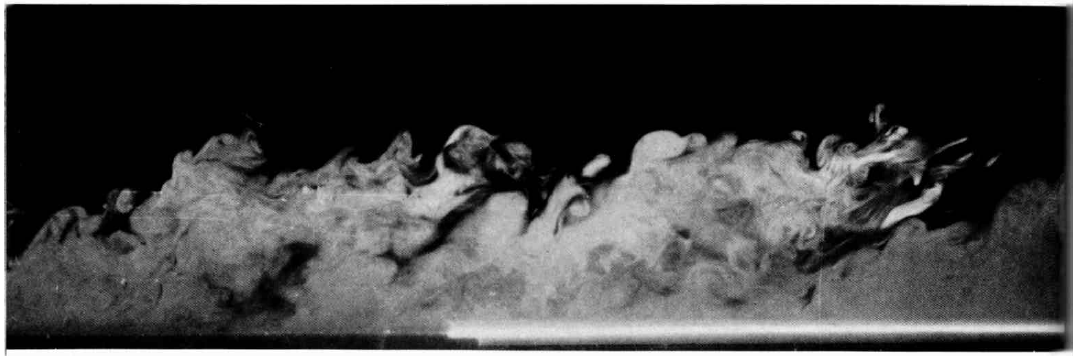
\includegraphics[width=\textwidth]{../fig/uitwendige_stroming/Turbulent_boundary_layer_Falco1977.png}\\
		\footnotesize{Bron: An Album of Fluid Motion (Van Dyke)}
  	\end{frame}
  	\begin{frame}
		\frametitle{Voorbeeld}
		\center
    	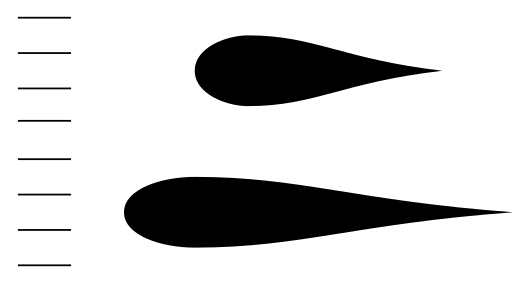
\includegraphics[width=\textwidth]{../fig/uitwendige_stroming/Oppervlakteweerstand}\\
  	\end{frame}
%%%%%%%%%%%%%%%%%%%%%%%%%%%%%%%%%%%%%%%%%%%%%%%%%%%%%%%%%%%%%%%%%%%%%%%%%%%
	\section{Grenslagen}
	\begin{frame}
		\frametitle{No-slip randvoorwaarde}
		\vspace{1cm}
		\center
		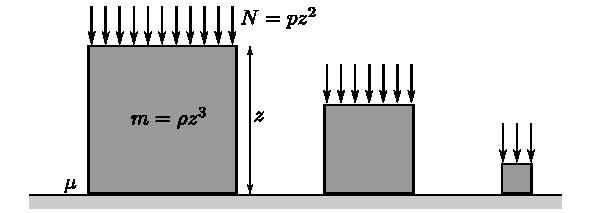
\includegraphics{../fig/uitwendige_stroming/No-slip_statische_wrijving}
		
		\pause
		\begin{equation*}
			m \frac{\diff v}{\diff t} = -\mu N
		\end{equation*}
  	\end{frame}
%%%%%%%%%%%%%%%%%%%%%%%%%%%%%%%%%%%%%%%%%%%%%%%%%%%%%%%%%%%%%%%%%%%%%%%%%%%
	\begin{frame}
		\frametitle{No-slip randvoorwaarde}
		\center
		\href{run:fig/uitwendige_stroming/No-Slip_condition.mp4}{
			\includegraphics[height=0.8\textheight]{../fig/uitwendige_stroming/No-Slip_condition.png}
		}\\
		\footnotesize{Bron: https://www.youtube.com/watch?v=cUTkqZeiMow}
  	\end{frame}
%%%%%%%%%%%%%%%%%%%%%%%%%%%%%%%%%%%%%%%%%%%%%%%%%%%%%%%%%%%%%%%%%%%%%%%%%%%	
  	\begin{frame}
		\frametitle{Het ontstaan van een grenslaag}
		\vspace{1cm}
		\center
		\only<1>{
			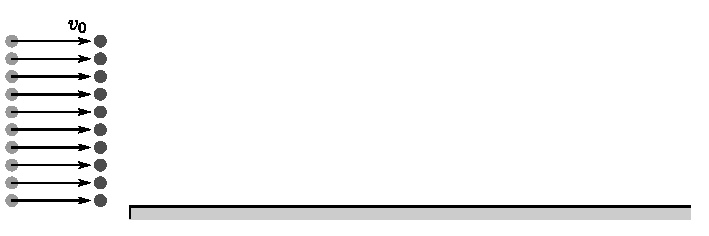
\includegraphics[width=\textwidth]{../fig/uitwendige_stroming/Laminaire_grenslaag0}
		}
		\only<2>{
			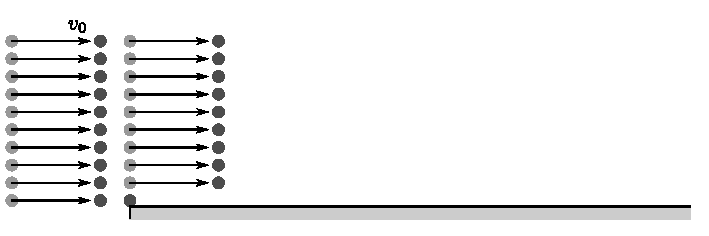
\includegraphics[width=\textwidth]{../fig/uitwendige_stroming/Laminaire_grenslaag1}
		}
		\only<3>{
			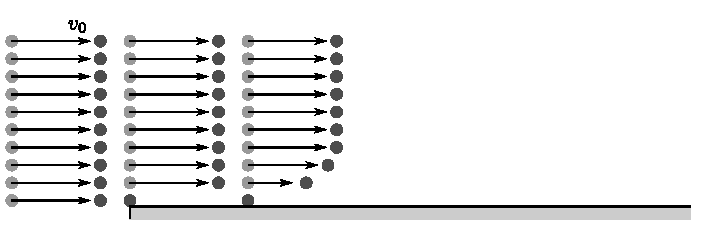
\includegraphics[width=\textwidth]{../fig/uitwendige_stroming/Laminaire_grenslaag2}
		}
		\only<4>{
			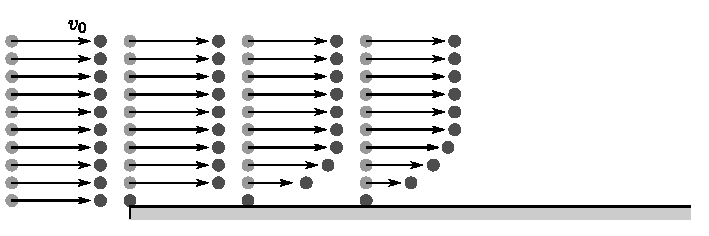
\includegraphics[width=\textwidth]{../fig/uitwendige_stroming/Laminaire_grenslaag3}
		}
		\only<5>{
			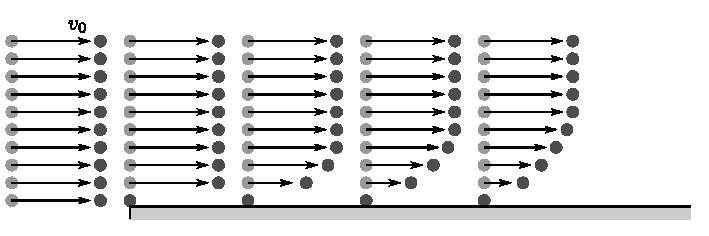
\includegraphics[width=\textwidth]{../fig/uitwendige_stroming/Laminaire_grenslaag4}
		}
		\only<6>{
			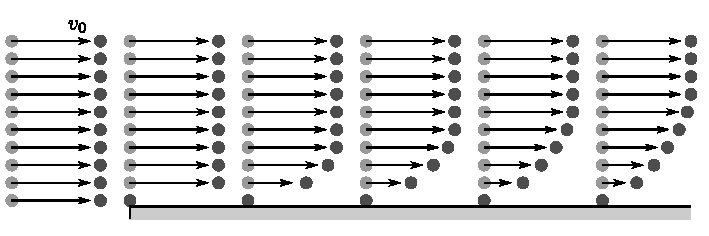
\includegraphics[width=\textwidth]{../fig/uitwendige_stroming/Laminaire_grenslaag5}
		}
		\only<7>{
			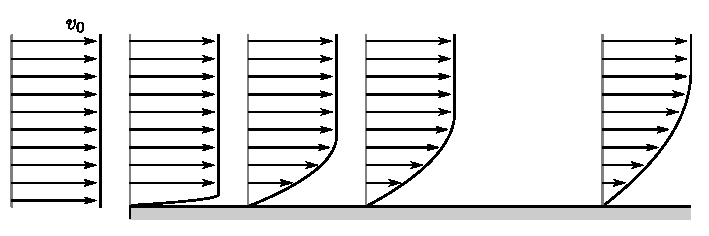
\includegraphics[width=\textwidth]{../fig/uitwendige_stroming/Laminaire_grenslaag6}
		}
		\only<8>{
			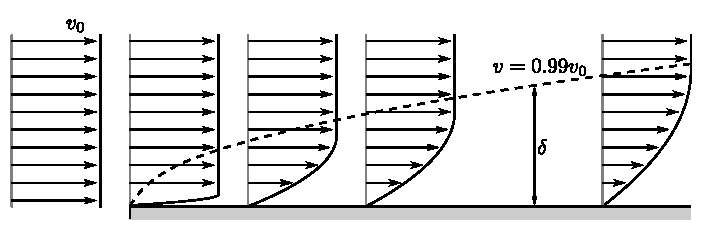
\includegraphics[width=\textwidth]{../fig/uitwendige_stroming/Laminaire_grenslaag}
		}
  	\end{frame}
%%%%%%%%%%%%%%%%%%%%%%%%%%%%%%%%%%%%%%%%%%%%%%%%%%%%%%%%%%%%%%%%%%%%%%%%%%%	
  	\begin{frame}
		\frametitle{Het ontstaan van een grenslaag}
		\center
		\href{run:fig/uitwendige_stroming/laminar_boundary_layer.mp4}{
			\includegraphics[width=\textwidth]{../fig/uitwendige_stroming/laminar_boundary_layer.png}
		}\\
		\footnotesize{Bron: https://www.youtube.com/watch?v=7SkWxEUXIoM}
  	\end{frame}
%%%%%%%%%%%%%%%%%%%%%%%%%%%%%%%%%%%%%%%%%%%%%%%%%%%%%%%%%%%%%%%%%%%%%%%%%%%
  	\begin{frame}
		\frametitle{Snelheidsprofiel}
		\begin{equation*}
			v_x \frac{\partial v_x}{\partial x} + v_y \frac{\partial v_x}{\partial y} = \nu \left( \frac{\partial^2 v_x}{\partial x^2} \right)
		\end{equation*}
		\pause
		\center
		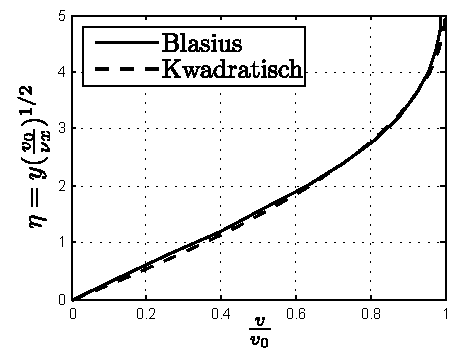
\includegraphics{../fig/uitwendige_stroming/Grenslaagsnelheid}
  	\end{frame}
%%%%%%%%%%%%%%%%%%%%%%%%%%%%%%%%%%%%%%%%%%%%%%%%%%%%%%%%%%%%%%%%%%%%%%%%%%%
  	\begin{frame}
		\frametitle{Impulsbalans in een laminaire grenslaag}
		\only<1>{
			\vspace{1cm}
			\center
			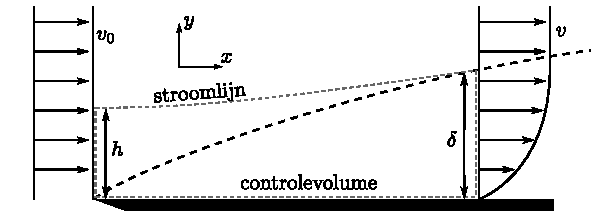
\includegraphics{../fig/uitwendige_stroming/Laminaire_grenslaag_controlevolume}
		}
		\only<2-6>{
			\begin{textblock}{5}(0,3)
           		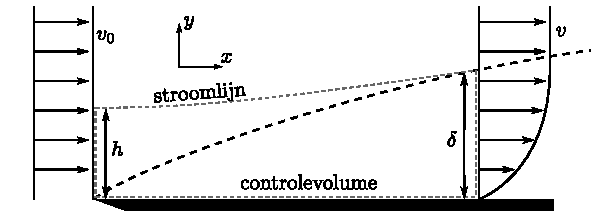
\includegraphics[width=5cm]{../fig/uitwendige_stroming/Laminaire_grenslaag_controlevolume}
        	\end{textblock}
        }
        \vspace{2cm}
        \only<2-4>{
        	\begin{equation*}
        		-F_d = \int_0^{\delta} \rho v(y)^2 b \diff y  - \int_0^{h} \rho v_0^2 b \diff y
        	\end{equation*}
        }
        \only<5-6>{
        	\begin{equation*}
        		-F_d = \int_0^{\delta} \rho v(y)^2 b \diff y  - \underlinered{\int_0^{h} \rho v_0^2 b \diff y}
        	\end{equation*}
        }
		\only<3>{
        	\begin{equation*}
        		\rho v_0 b h = \int_0^{\delta} \rho v(y) b \diff y
        	\end{equation*}
        }
        \only<4>{
        	\begin{equation*}
        		\rho v_0^2 b h = \int_0^{\delta} \rho v_0 v(y) b \diff y
        	\end{equation*}
        }
        \only<5-6>{
        	\begin{equation*}
        		\underlinered{\rho v_0^2 b h} = \int_0^{\delta} \rho v_0 v(y) b \diff y
        	\end{equation*}
        }
		\only<6-6>{
			\vspace{0.5cm}
        	\begin{equation*}
        		F_d = \rho b \int_0^{\delta} v(y)(v_0-v(y))\diff y
        	\end{equation*}
        }
  	\end{frame}
%%%%%%%%%%%%%%%%%%%%%%%%%%%%%%%%%%%%%%%%%%%%%%%%%%%%%%%%%%%%%%%%%%%%%%%%%%%
	\section{Turbulentie}	
  	\begin{frame}
		\frametitle{Turbulente grenslaag}
		\vspace{1cm}
		\center
		\only<1>{
			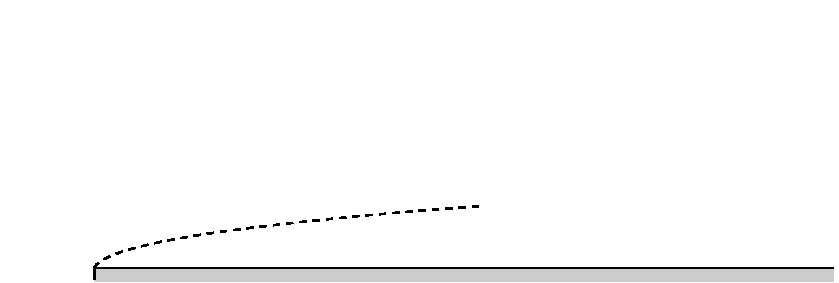
\includegraphics[width=\textwidth]{../fig/uitwendige_stroming/Turbulente_grenslaag0}
		}
		\only<2>{
			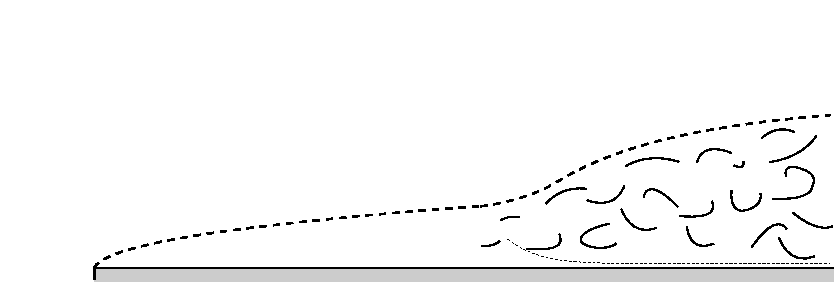
\includegraphics[width=\textwidth]{../fig/uitwendige_stroming/Turbulente_grenslaag1}
		}
		\only<3>{
			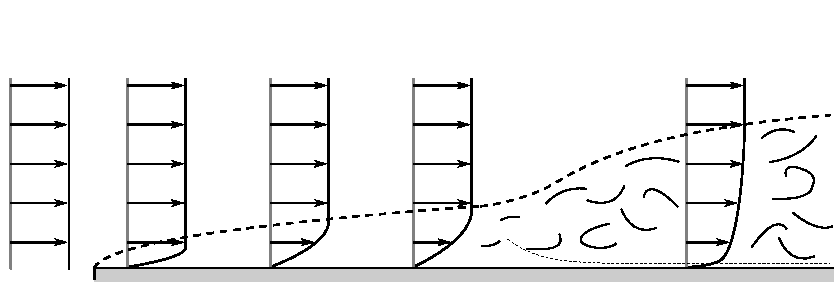
\includegraphics[width=\textwidth]{../fig/uitwendige_stroming/Turbulente_grenslaag2}
		}
		\only<4>{
			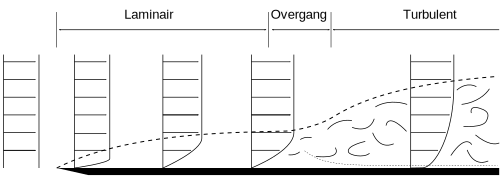
\includegraphics[width=\textwidth]{../fig/uitwendige_stroming/Turbulente_grenslaag}
		}
  	\end{frame}
%%%%%%%%%%%%%%%%%%%%%%%%%%%%%%%%%%%%%%%%%%%%%%%%%%%%%%%%%%%%%%%%%%%%%%%%%%%
  	\begin{frame}
		\frametitle{Turbulentie}
		\center
		\begin{tabular}{cc}
			\href{run:fig/uitwendige_stroming/Turbulent_mixing.mp4}{
				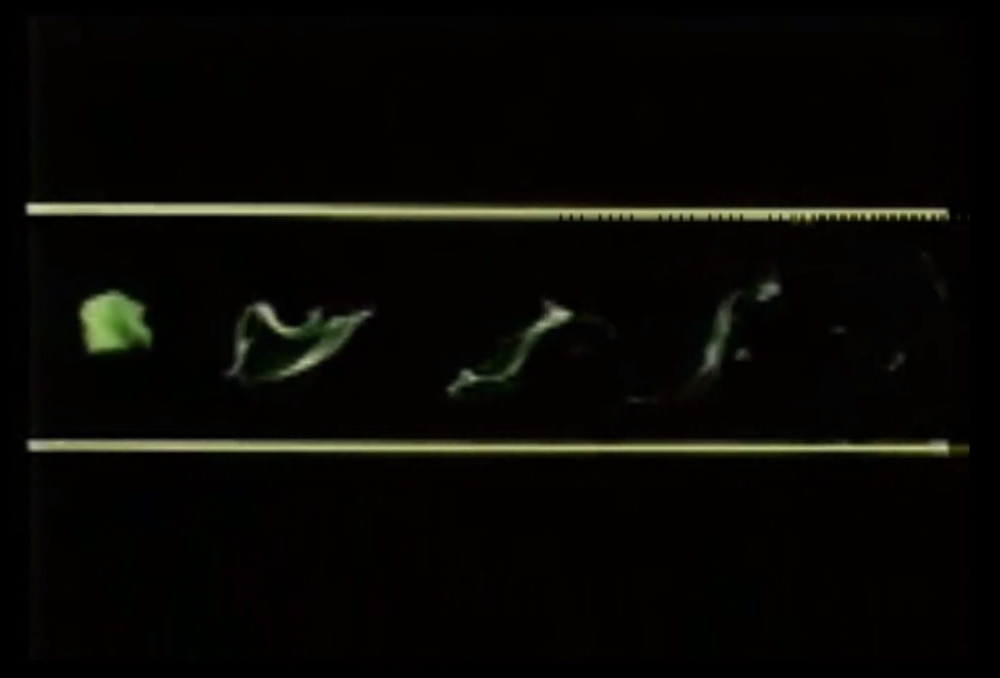
\includegraphics[height=0.3\textheight]{../fig/uitwendige_stroming/Turbulent_mixing.png}
			}
			&
			\href{run:fig/uitwendige_stroming/Turbulent_boundary_layer_eddies.mp4}{
				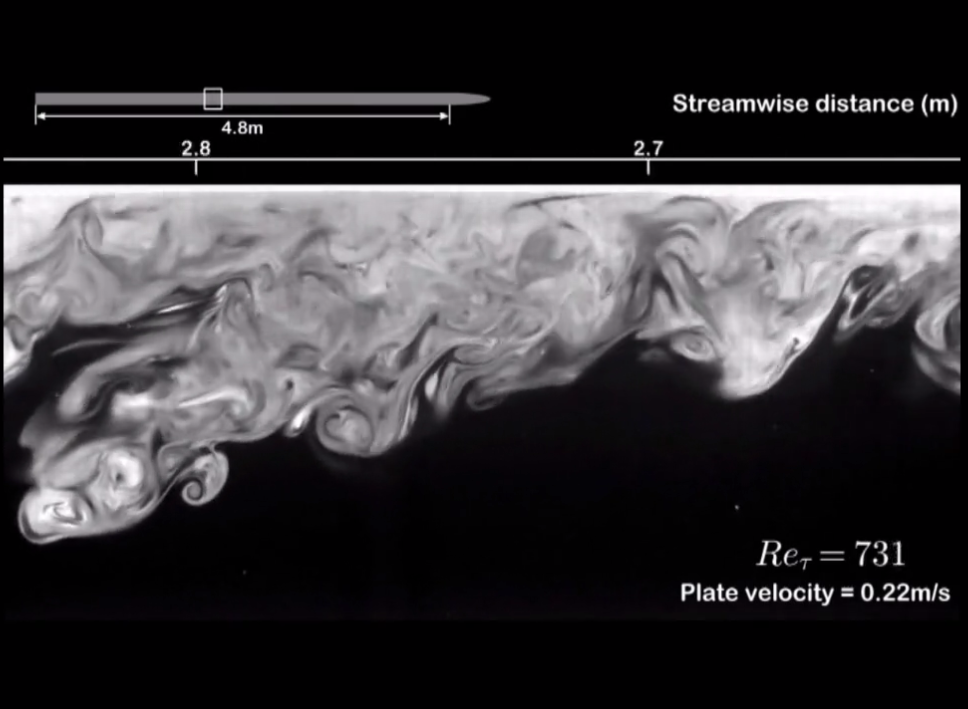
\includegraphics[height=0.3\textheight]{../fig/uitwendige_stroming/Turbulent_boundary_layer_eddies.png}
			}
			\\
			&
			\\
			\href{run:fig/uitwendige_stroming/Turbulent_velocity_profile.mp4}{
				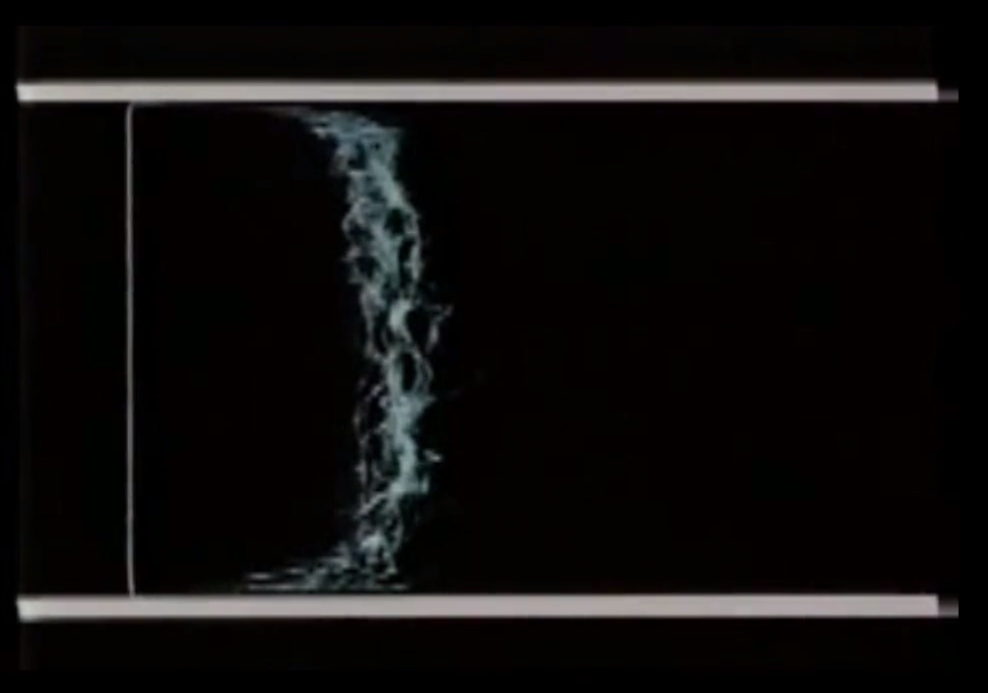
\includegraphics[height=0.3\textheight]{../fig/uitwendige_stroming/Turbulent_velocity_profile.png}
			}
			&
			\href{run:fig/uitwendige_stroming/Turbulent_laminar_velocity_profile.mp4}{
				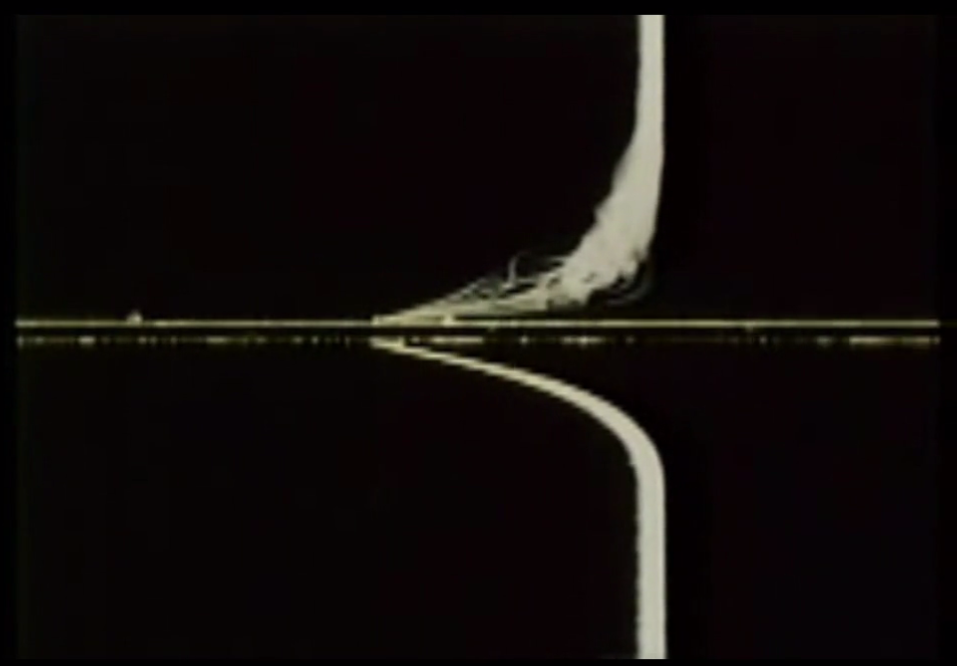
\includegraphics[height=0.3\textheight]{../fig/uitwendige_stroming/Turbulent_laminar_velocity_profile.png}
			}
		\end{tabular}\\
		
		\footnotesize{Bron: https://www.youtube.com/watch?v=1\_oyqLOqwnI}\\
		\footnotesize{Bron: https://www.youtube.com/watch?v=e1TbkLIDWys}
		\footnotesize{Bron: https://www.youtube.com/watch?v=wMxK2GtFFq0}
  	\end{frame}
%%%%%%%%%%%%%%%%%%%%%%%%%%%%%%%%%%%%%%%%%%%%%%%%%%%%%%%%%%%%%%%%%%%%%%%%%%%
  	\begin{frame}
		\frametitle{Turbulentie}
		\vspace{1cm}
		\begin{itemize}
			\pause
			\item Schijnbaar willekeurig
			\pause
			\item Zeer gevoelig aan begincondities
			\pause
			\item Menging
			\pause
			\item Variatie in tijd en lengte schalen
			\pause
			\item 3 dimensionaal
		\end{itemize}
  	\end{frame}
%%%%%%%%%%%%%%%%%%%%%%%%%%%%%%%%%%%%%%%%%%%%%%%%%%%%%%%%%%%%%%%%%%%%%%%%%%%
	\begin{frame}
		\frametitle{Laminaire stroming}
		\center
		\href{run:fig/uitwendige_stroming/Laminar_flow_mixing.mp4}{
			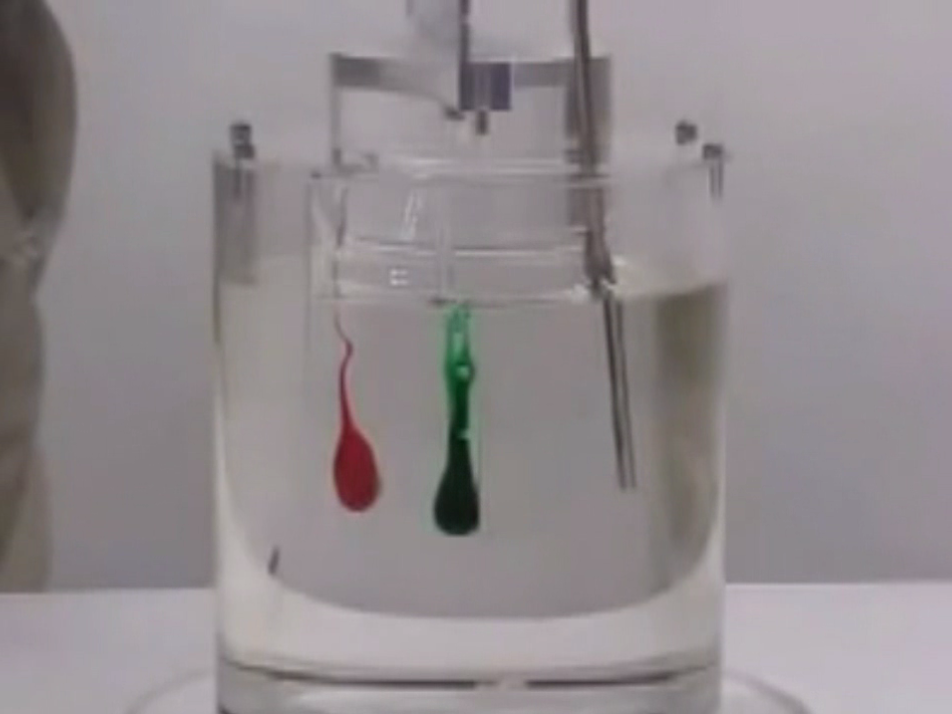
\includegraphics[height=0.8\textheight]{../fig/uitwendige_stroming/Laminar_flow_mixing.png}
		}\\
		\footnotesize{Bron: https://www.youtube.com/watch?v=p08\_KlTKP50}
  	\end{frame}
%%%%%%%%%%%%%%%%%%%%%%%%%%%%%%%%%%%%%%%%%%%%%%%%%%%%%%%%%%%%%%%%%%%%%%%%%%%
  	\begin{frame}
		\frametitle{Energiecascade}
		\only<1-2>{
			\begin{align*}
				&\rho \left(\frac{\partial v_x}{\partial t} + v_x \frac{\partial v_x}{\partial x} + v_y \frac{\partial v_x}{\partial y} + v_z \frac{\partial v_x}{\partial z} \right) = \nonumber\\
				&\hspace{2cm} -\frac{\partial p}{\partial x} +\rho g_x + \mu \left( \frac{\partial^2 v_x}{\partial x^2} + \frac{\partial^2 v_x}{\partial y^2} + \frac{\partial^2 v_x}{\partial z^2} \right)
			\end{align*}
		}
		\only<3-4>{
			\begin{align*}
				&\rho \left(\frac{\partial v_x}{\partial t} + \underlinered{v_x \frac{\partial v_x}{\partial x}} + v_y \frac{\partial v_x}{\partial y} + v_z \frac{\partial v_x}{\partial z} \right) = \nonumber\\
				&\hspace{2cm} -\frac{\partial p}{\partial x} +\rho g_x + \mu \left( \frac{\partial^2 v_x}{\partial x^2} + \frac{\partial^2 v_x}{\partial y^2} + \frac{\partial^2 v_x}{\partial z^2} \right)
			\end{align*}
		}
		\only<2-4>{
		
			Stel:
			\begin{equation*}
				v_x = \sin{\omega x}
			\end{equation*}
		}
		\only<3-4>{
			Dan:
			\begin{equation*}
				v_x \frac{\partial v_x}{\partial x} = \omega \sin(\omega x) \cos(\omega x) = \frac{1}{2} \omega \sin( 2 \omega x) 
			\end{equation*}
		}
  	\end{frame}
%%%%%%%%%%%%%%%%%%%%%%%%%%%%%%%%%%%%%%%%%%%%%%%%%%%%%%%%%%%%%%%%%%%%%%%%%%%
  	\begin{frame}
		\frametitle{Energiecascade}
		\vspace{1cm}
		\center
		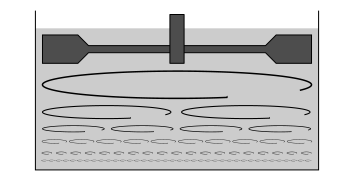
\includegraphics{../fig/uitwendige_stroming/Energie_cascade}
  	\end{frame}
%%%%%%%%%%%%%%%%%%%%%%%%%%%%%%%%%%%%%%%%%%%%%%%%%%%%%%%%%%%%%%%%%%%%%%%%%%%
  	\begin{frame}
		\frametitle{Turbulentie en het Reynoldsgetal}
		\vspace{1cm}
		\begin{equation*}
			\text{Re} = \dfrac{v x}{\nu} = \dfrac{\text{traagheidskracht}}{\text{viskeuze krachten}}
		\end{equation*}
		
		\vspace{1cm}
		Dus
		\center
		\vspace{0.5cm}
		\pause
		Re klein $\Longrightarrow$ Laminair
		
		\vspace{0.5cm}
		\pause
		Re groot $\Longrightarrow$ Turbulent 
  	\end{frame}
%%%%%%%%%%%%%%%%%%%%%%%%%%%%%%%%%%%%%%%%%%%%%%%%%%%%%%%%%%%%%%%%%%%%%%%%%%%
\end{document}